\documentclass[titlepage, 12pt]{article}

\title{

\includegraphics[width=.3\textwidth]{cvut-logo.jpg}\par
\vspace{10mm}
\indent
\textbf{CZECH TECHNICAL UNIVERSITY IN PRAGUE}

FACULTY OF TRANSPORT SCIENCES

\vfill

{\Large JAN MACEK}
\vspace{10mm}

AGENT-BASED MODELING OF ITS SYSTEMS IN VEHICLE SIMULATOR 
\vspace{15mm}

{\Large MASTER'S THESIS}
\vfill

}
\date{\Large 2022}

\usepackage[utf8]{inputenc}
\usepackage[T1]{fontenc}
% \usepackage{cm-super}
\usepackage{listings}
\usepackage{fancyhdr}
\usepackage{graphicx}
\usepackage{parskip}
\usepackage{svg}
\usepackage[a4paper, top=25mm, bottom=25mm, left=30mm, right=20mm, twoside]{geometry}
\usepackage{tabularx}
\usepackage{caption}
\usepackage{hyperref}
\usepackage{xcolor}
\usepackage{amsmath}
\usepackage[sorting=none]{biblatex} 
\usepackage{color}
\usepackage{pdfpages}
\usepackage{enumitem}
\usepackage{amssymb}
\usepackage{booktabs}
\usepackage{microtype}
\usepackage{subfiles}
\usepackage{multirow}
\usepackage{pdfpages}
\usepackage{enumitem}
\usepackage{soul}

\definecolor{dkgreen}{rgb}{0,0.6,0}
\definecolor{gray}{rgb}{0.5,0.5,0.5}
\definecolor{mauve}{rgb}{0.58,0,0.82}
\definecolor{inline}{rgb}{0.25,0.25,0.80}


\addbibresource{references.bib}

\hypersetup{
    colorlinks,
    linkcolor={red!50!black},
    citecolor={blue!50!black},
    urlcolor={blue!70!black}
}

\pagestyle{fancy}

\graphicspath{{./img}}

\fancyhead[L]{Jan Macek}
\setlength{\headheight}{15pt}

\newlength{\varSepscale}
\setlength{\varSepscale}{16pt}
\newcommand{\itemspacing}[1]{\setlength\itemsep{\dimexpr #1\varSepscale-\varSepscale}}
\newcommand{\term}[1]{\hspace*{2em}\textit{#1}\, -\,}
\newcommand{\rot}[1]{\rotatebox[origin=c]{90}{#1}}
\newcommand{\talign}[3]{\makebox[#2em]{#1\hfill}#3}

%DOCUMENT
\begin{document}
\setlength{\baselineskip}{1.5em}
\maketitle

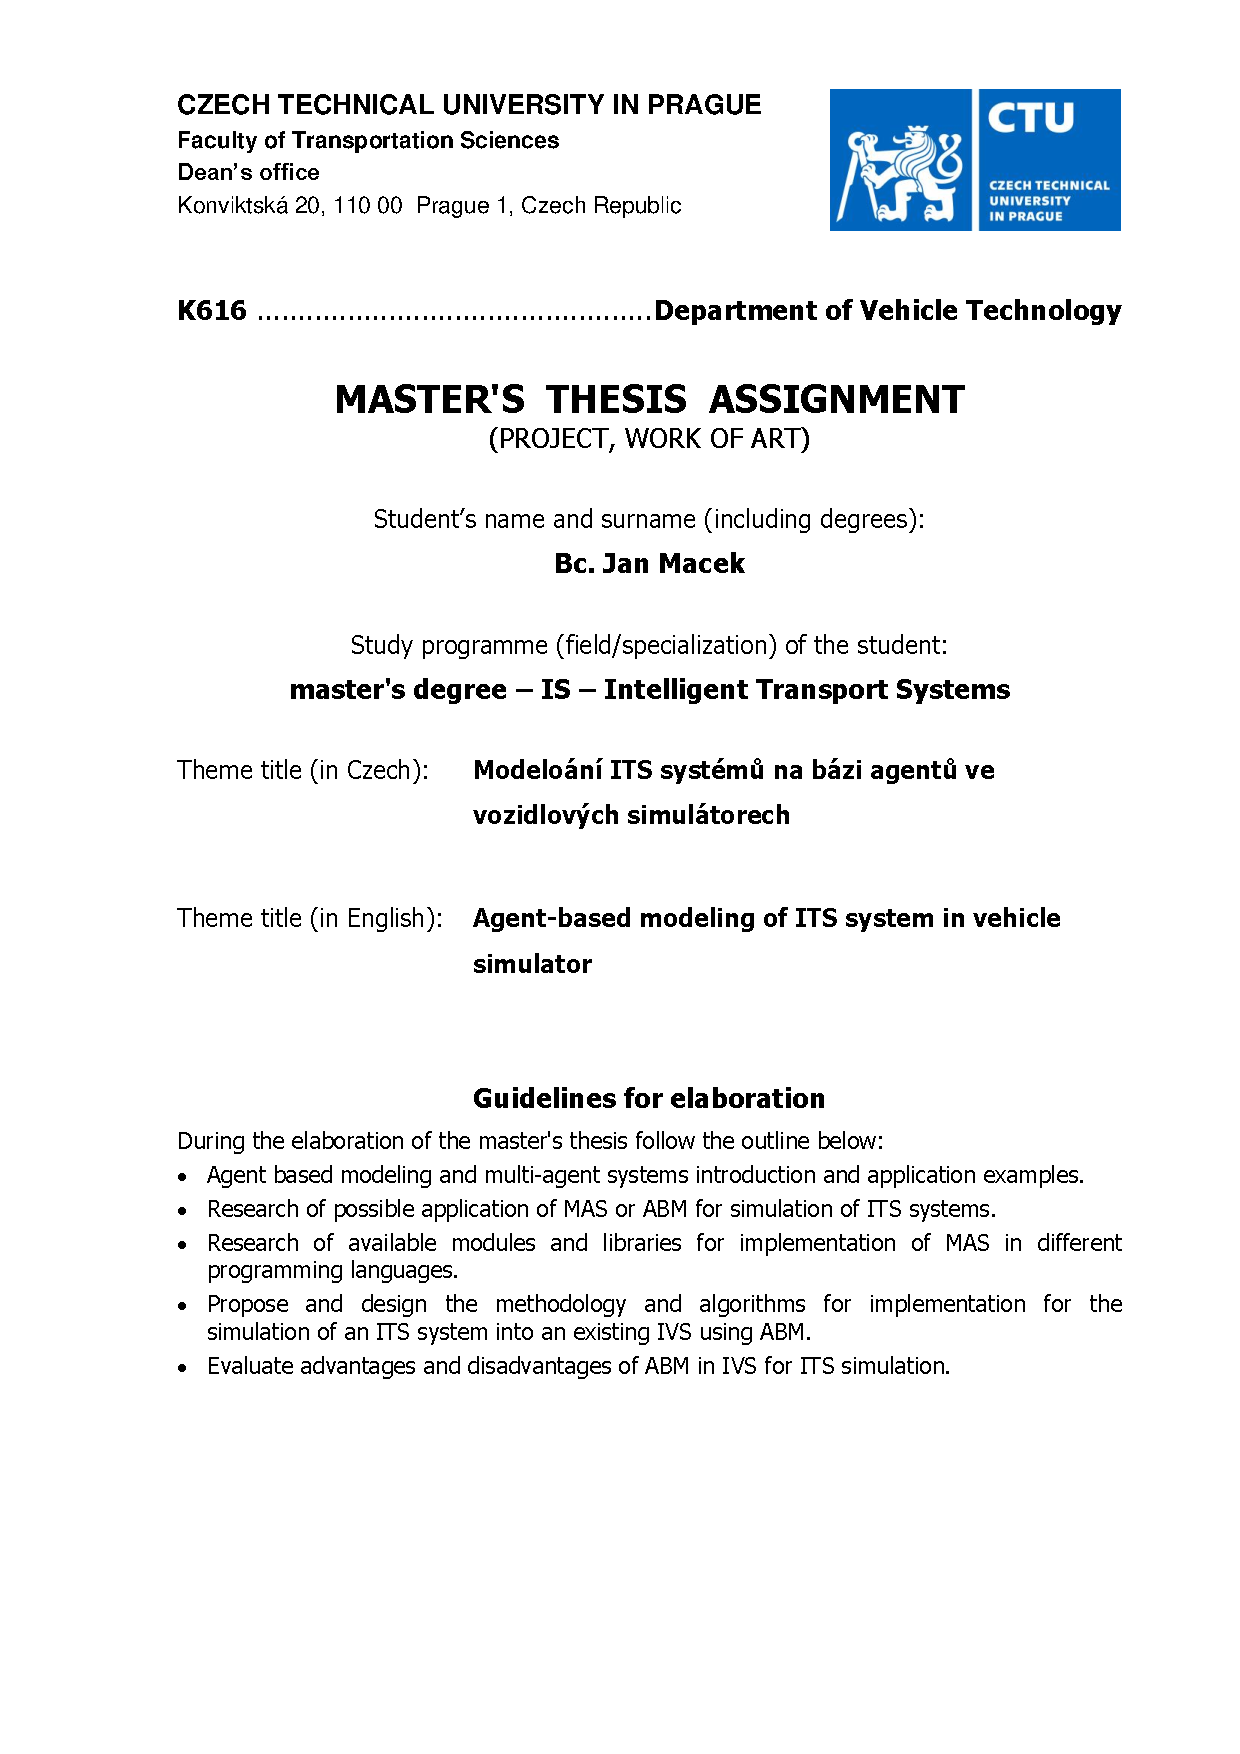
\includepdf[pages=-]{zadani-dp-jan-macek.pdf}

\begin{abstract}
    The use of Intelligent Transport Systems (ITS) has become increasingly important in
    managing transportation networks and improving safety, efficiency, and sustainability. This
    research aims to advance the development of ITS through the application of Multi-agent Systems (MAS)
    in a vehicle simulator. The opportunities and underlying challenges of successfully performing a 
    simulation of an ITS system in a vehicle simulator are investigated and consequentially, a 
    framework for ITS solution implementation into a simulator software is presented. The agent-based 
    framework is able to facilitate simulating complex behaviour of various road users as well as 
    road equipment such as (cooperative) traffic lights. The main advantages of the framework are 
    modularization of agent's skills which makes it easier to model complex behaviour. The framework 
    also simplifies implementation of communication interface to arbitrary agent, making it a strong tool 
    for simulating Cooperative ITS (C-ITS). In the last part of the thesis, a simple ITS solution is 
    successfully developed using the framework, which features a connected traffic light which provides 
    information to connected vehicles for dynamic navigation. The framework can enable vehicle simulator 
    developers to be able to implement various Intelligent Transport Systems into vehicle
    simulator software while reducing development time and increasing maintainability of the software.
 \end{abstract}

\tableofcontents
\listoftables
\listoffigures
\newpage

\section{Introduction}

Simulating traffic in a virtual environment, such as an Interactive Vehicle Simulator (IVS), is
a complex problem, mainly because of its highly dynamic nature. Trying to accurately simulate
traffic on a microscopic level, where individual road users (e.g. vehicles) are the elementary
units in a system requires complex modelling.  All vehicles need to interact with each other
and act upon other drivers' actions. Because agent-based simulations have proven to model
complex behavior well, this modeling technique seems like a suitable solution for achieving a
realistic traffic environment for IVS. This thesis aims to investigate the possibilities and
delimitations of multi-agent systems application(s) for Intelligent Transport Systems (ITS)
modeling in an IVS. 

In the first two chapters, a review of the state-of-art research on Intelligent Transport
Systems and Multi-agent Systems (MAS) are presented, discussing the important features related
to the main topic of the thesis. This research leads to the definition of system requirements
that are described in the third chapter. In the fourth section, a framework architecture model
is proposed, in line with MAS paradigms and adapted for ITS solutions simulation. In the fifth
section, the usage and requirements of tools for framework development are discussed, mainly
describing the simulator software integration and additional development platforms and
libraries that could potentially facilitate the framework design process. In the sixth section,
a technical implementation of the framework is presented, showing the implementation details
while also serving as the software's documentation. In section number seven, a validation of
the proposed system is conducted by implementing a distributed cooperative ITS system into the
IVS, using the proposed framework and assessing its performance and overall results.

\subsection{Introduction to the problem}

In a world where vehicle transport plays an inseparable role in society, with an ever-increasing
demand, it is important to analyze and study driver behavior and inherently interactions and
relationships between drivers and their surroundings. This is supported by the fact that, even though
substantial advancements in autonomous driving are being made, for the near future, vehicles 
will be controlled by humans and therefore be exposed to a substantial risk of danger. 
Data shows that about 95 \% of traffic accidents are a result of human error \cite{Parliament2021}. 
Each traffic accident has got a tremendous effect on socioeconomic growth. A study by the European
Union states that accident-related expenses (including the cost of a fatality) cost 1,8 \% of EU GDP \cite{Wijnen2017}.  
A rather non-cynical point of view is that each life lost is a failure in society itself and an effort
should be made to eliminate fatal accidents.

A method that has proven to be effective at studying driver behavior and traffic safety is by
using interactive vehicle simulators (IVS), which allow to undertake experiments in a safe,
controlled and reproducible way \cite{Winter2012}.  Because the driving simulator is a digital
twin of a real vehicle, it is naturally reasonable to make the interaction between the driver
and IVS as close to reality as possible, which inherently improves the trustworthiness of
acquired data from experiments and potentially also the range of IVS applications. The IVS has
got a broad spectrum of utilization. It is not only used as a tool to research driver
behaviour, but also used in development and testing of advanced driver-assistance systems,
extending the simulator to a hardware-in-the-loop or vehicle-in-the-loop software, which
enables testing real hardware and simulating full road testing \cite{Horvath2019}.

\subsection{Aim}

The goal of this thesis is to investigate multi-agent systems (MAS) and their principles and
evaluate the usages of these systems related to Intelligent Transport Systems (ITS) research,
where their shared characteristics of distributed interoperability make agent-based modeling a
strong tool for simulating ITS solutions. The output of the experimental/practical part of the
thesis is a MAS-based simulation framework for facilitating the process of ITS solutions
simulation with the benefit of modular and fast extensibility.  The developed system should
also be able to model state-of-the-art ITS systems that utilize communication between road
users, such as C-ITS systems. 

 \subsection{Research questions}

In order to evaluate the research, the following questions are given that the thesis should answer, which are following up on the thesis assignment. 

% \begin{itemize}
%     \item Agent-based modeling and multi-agent systems introduction and application examples
%     \item Research of possible application of MAS or ABM for simulation of ITS systems
%     \item Research of available modules and libraries for implementation of MAS in different programming languages
%     \item Propose and design a methodology and algorithms for implementation for the simulation of an ITS into an existing IVS using ABM
%     \item Evaluate advantages and disadvantages of ABM in IVS for ITS simulation
% \end{itemize}

\begin{itemize}
    \item Can agent-based modeling be applied to simulate Intelligent Transport Systems in vehicle simulators and are they a viable option?
    \item How would an ITS simulation be implemented into an existing IVS using agent-based modelling?
    \item What are the available modules and libraries for implementing MAS in different programming languages?
    \item What are the advantages and challenges associated with using agent-based modeling to simulate Intelligent Transport Systems in vehicle simulators, and how can they be addressed?
\end{itemize}

% \begin{itemize}
% \end{itemize}

\subsection{Methodology}

The main objective of the thesis is to create a module for ITS implementation into a vehicle simulator software. 
The first step will be to perform a literature review regarding the main thesis topics - Multi-agent Systems and 
Intelligent Transport Systems. By reviewing MAS, insight will be gained into how to approach modeling systems using 
such a paradigm. Secondly, research on the current state of Intelligent Transport Systems will be conducted in 
order to identify system features and interactions that are important when attempting to create a 
base model for ITS implementation. 

After gathering and analyzing resources for creating the model, requirements for the model will be defined to consolidate 
the gathered information regarding the topic. Based on the defined requirements, an implementation framework/model will be 
defined. Mainly, its individual components will be described and relations between the components and their rules will be 
described as well. 

After the model structure definition, implementation into the simulator software will be discussed and executed. 
The goal is to define and implement a module/framework for general ITS implementation in a vehicle simulator. 
The main objective of the framework development will be to create a framework that will be sufficiently modular for 
a wide variety of ITS solutions to implement and at the same time provide sufficient support for the user when 
implementing a specific system using the framework. The capability of the developed framework will be validated
by implementing a sample ITS solution, which will help evaluate the overall implementation process and the 
model's capabilities and shortcomings.

\subsection{Delimitations}

Research delimitations refer to the scope of the study. The delimitations
for a thesis on Agent-based modeling of Intelligent Transport Systems in vehicle simulator include mainly 
the technical scope. The framework will need to be compatible with the Unity game development engine which 
is used in the IVS laboratories of the Czech Technical University University in Prague (CTU). It should be well-integrated with the simulator software so that 
the development using the framework will offer seamless interaction with other components of the simulator software. 


\subfile{1its}

\subfile{2mas}

\subfile{3requirements}

\subfile{4toolset}

\subfile{5system}

\subfile{6implementation}

\subfile{7validation}

\subfile{8discussion.tex}

\clearpage

\section{Conclusion}

ITS solutions are often systems integrating a large number of 
actors in a highly dynamic environment. In recent times, modern engineering made it possible 
to equip mobile devices, including road vehicles, with high-performance computers, making 
distributed intelligence a promising field for research, including Intelligent Transport Systems 
research.

The goal of this thesis was to investigate Multi-Agent Systems, which is a sub-field of Artificial Intelligence 
research, especially research related to the application of Multi-Agent Systems in Intelligent Transport Systems 
simulation. 

First, the area of Intelligent Transport Systems was investigated, setting delimitations and important features 
that were important to the topic of the thesis. The relationship between IVS and ITS systems was discussed, leading 
to a discussion about intelligence distribution and current research in the ITS field. 

The second part was dedicated to MAS literature review and the main principles of MAS were discussed. Furthermore, MAS 
individual MAS architectures were described and reviewed. Finally, the concepts of communication between agents were investigated,
defining requirements on how the agents should communicate. 

In the practical part of the thesis, delimitations and system requirements were defined first in order to facilitate the 
process of implementation and clearly define the system's capabilities. The development platform was briefly discussed, 
going over the options for potential facilitation of the implementation of the proposed system. It was identified that 
there are no suitable modules for MAS implementation to an IVS, as the research modules were either outdated or focused on 
different aspects of multi-agent systems. Therefore, it was decided that the framework would be built from the ground up.

Next, the actual system was proposed. The system design was divided into two parts - a
micro-architecture that focused on the inner structure of individual agents, whose goal was to
make the agents sufficiently modular as well as to actually facilitate the ITS implementation.
The architecture was designed based on the literature review in the preceding chapters. The
second part was dedicated to the macro architecture, which described how the individual agents
should interact with each other. The integral part of agent interaction was communication
specification, how agents will send and receive information.  Based on the preceding research
on ITS and MAS, the ETSI messaging standards (CAM \& DENM) were decided to be implemented.

After the system for MAS-based ITS systems implementation has been specified, the next part was
devoted to the system implementation.  The outcome is a highly modular framework that is
integrated with the chosen simulator software, with general behavior specific to MAS \& ABM 
and the architecture pre-implemented. The framework was implemented using the C\# programming 
language and the simulator engine (Unity) API. 

The developed framework was then validated by choosing a case appropriate for demonstration of the 
framework's utility. The case was chosen to be a dynamic routing system whose purpose was to 
improve traffic conditions by harmonizing a road network's load by the use of cooperative 
traffic lights and connected vehicles. The system was successfully implemented and the analysis of the 
simulation showed that the system is behaving as expected, i.e. reducing the overall travel time when 
calibrated.

Overall, the goals specified by the thesis guidelines have been fulfilled. The outcome of the thesis is a 
modular C\# framework/module which facilitates implementation of various (Cooperative) 
Intelligent Transport Systems solutions implementation into a vehicle simulator software. 

\clearpage

\thispagestyle{empty}

\clearpage

\printbibliography
\end{document}
